\begin{figure}[htbp]
\section*{ NKX6-2}
\centering
\begin{subfigure}[b]{0.95\textwidth}
\centering
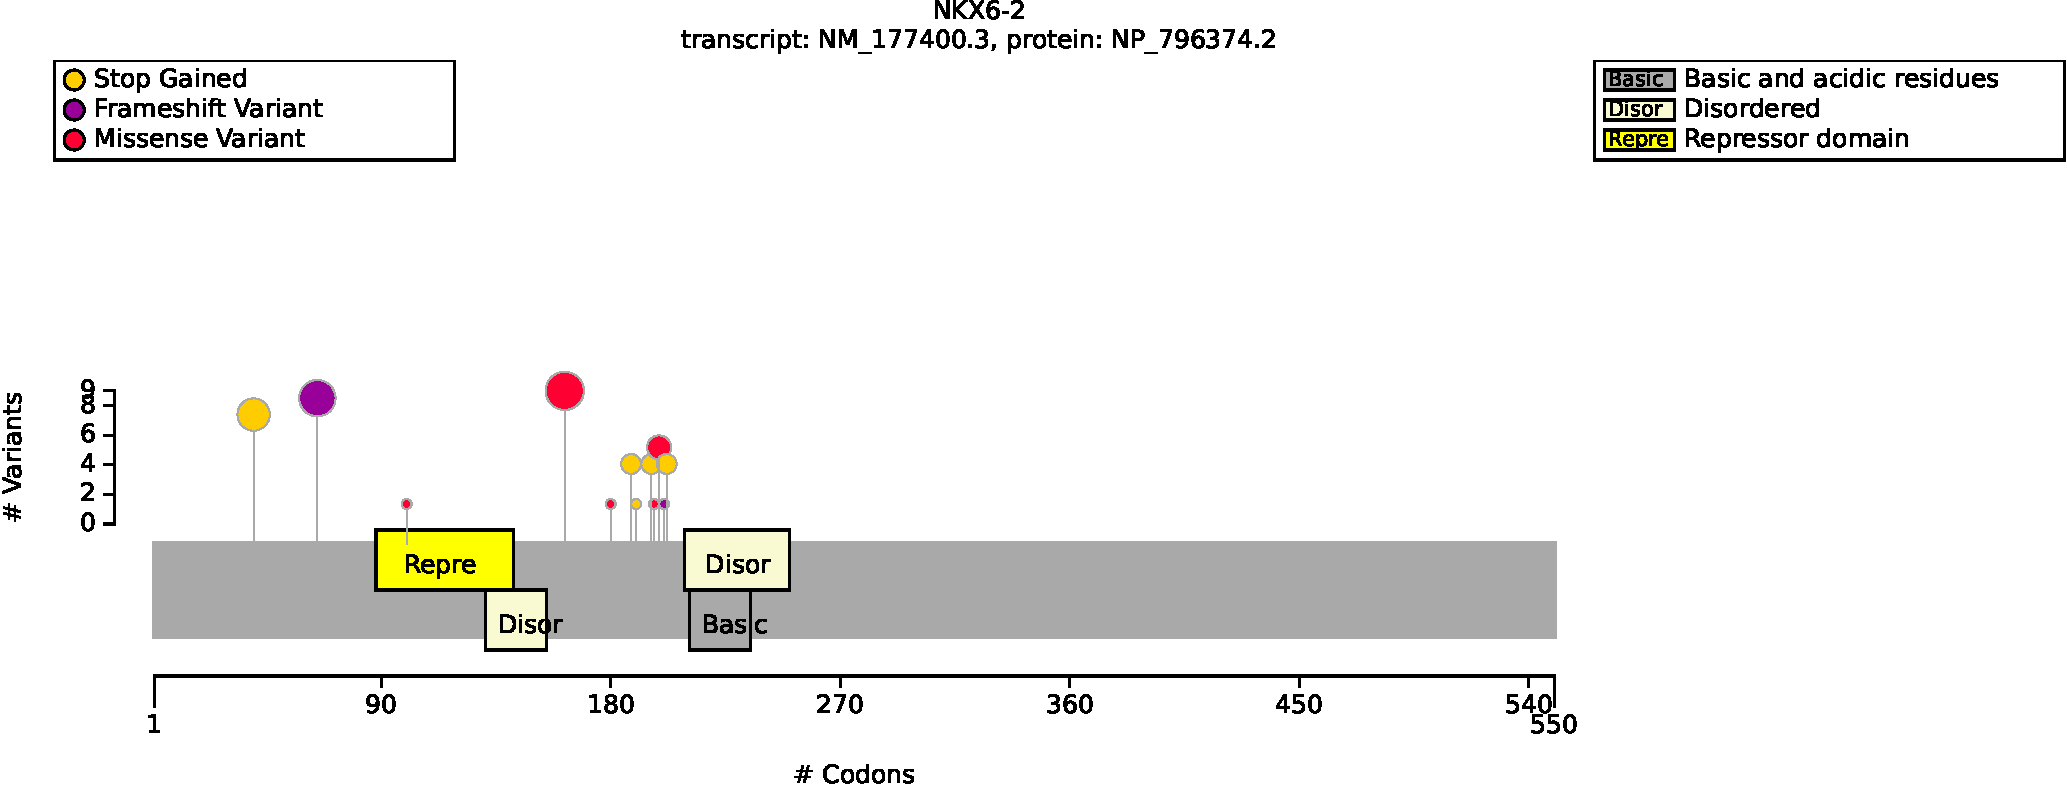
\includegraphics[width=\textwidth]{ img/NKX6-2_protein_diagram.pdf} 
\captionsetup{justification=raggedright,singlelinecheck=false}
\caption{Distribution of variants in NKX6-2}
\end{subfigure}

\vspace{2em}

\begin{subfigure}[b]{0.95\textwidth}
\centering
\resizebox{\textwidth}{!}{
\begin{tabular}{llllrr}
\toprule
Genotype (A) & Genotype (B) & total tests performed & significant results\\
\midrule
missense/missense & other/other OR missense/other & 21 & 0\\
L163V/L163V & L163V/other OR other/other & 21 & 0\\
N term/N term OR N term/other & other/other & 21 & 0\\
FEMALE & MALE & 21 & 0\\
\bottomrule
\end{tabular}
}
\captionsetup{justification=raggedright,singlelinecheck=false}
\caption{             Fisher Exact Test performed to compare HPO annotation frequency with respect to genotypes. }
\end{subfigure}

\vspace{2em}

\caption{ The cohort comprised 33 individuals (15 females, 18 males). A total of 39 HPO terms were used to annotate the cohort. Disease diagnosis: Spastic ataxia 8, autosomal recessive, with hypomyelinating leukodystrophy (OMIM:617560). No statistically significant results identified. A total of 13 unique variant alleles were found in \textit{NKX6-2} (transcript: \texttt{NM\_177400.3}, protein id: \texttt{NP\_796374.2}).}
\end{figure}
